\section{Classification} \label{sec:classfication}

Clustering was our first approach as an unsupervised algorithm seemed
to best fit the data at hand. As such, we tried the following methods,
all of which are inbuilt in scikit-learn:\\

\begin{itemize}
\item K-Means
\item Affinity Propagation
\item Mean-Shift
\item Ward Agglomerative Clustering
\item DBSCAN
\end{itemize}

\begin{figure*}[h!]
    \centering
    \fbox{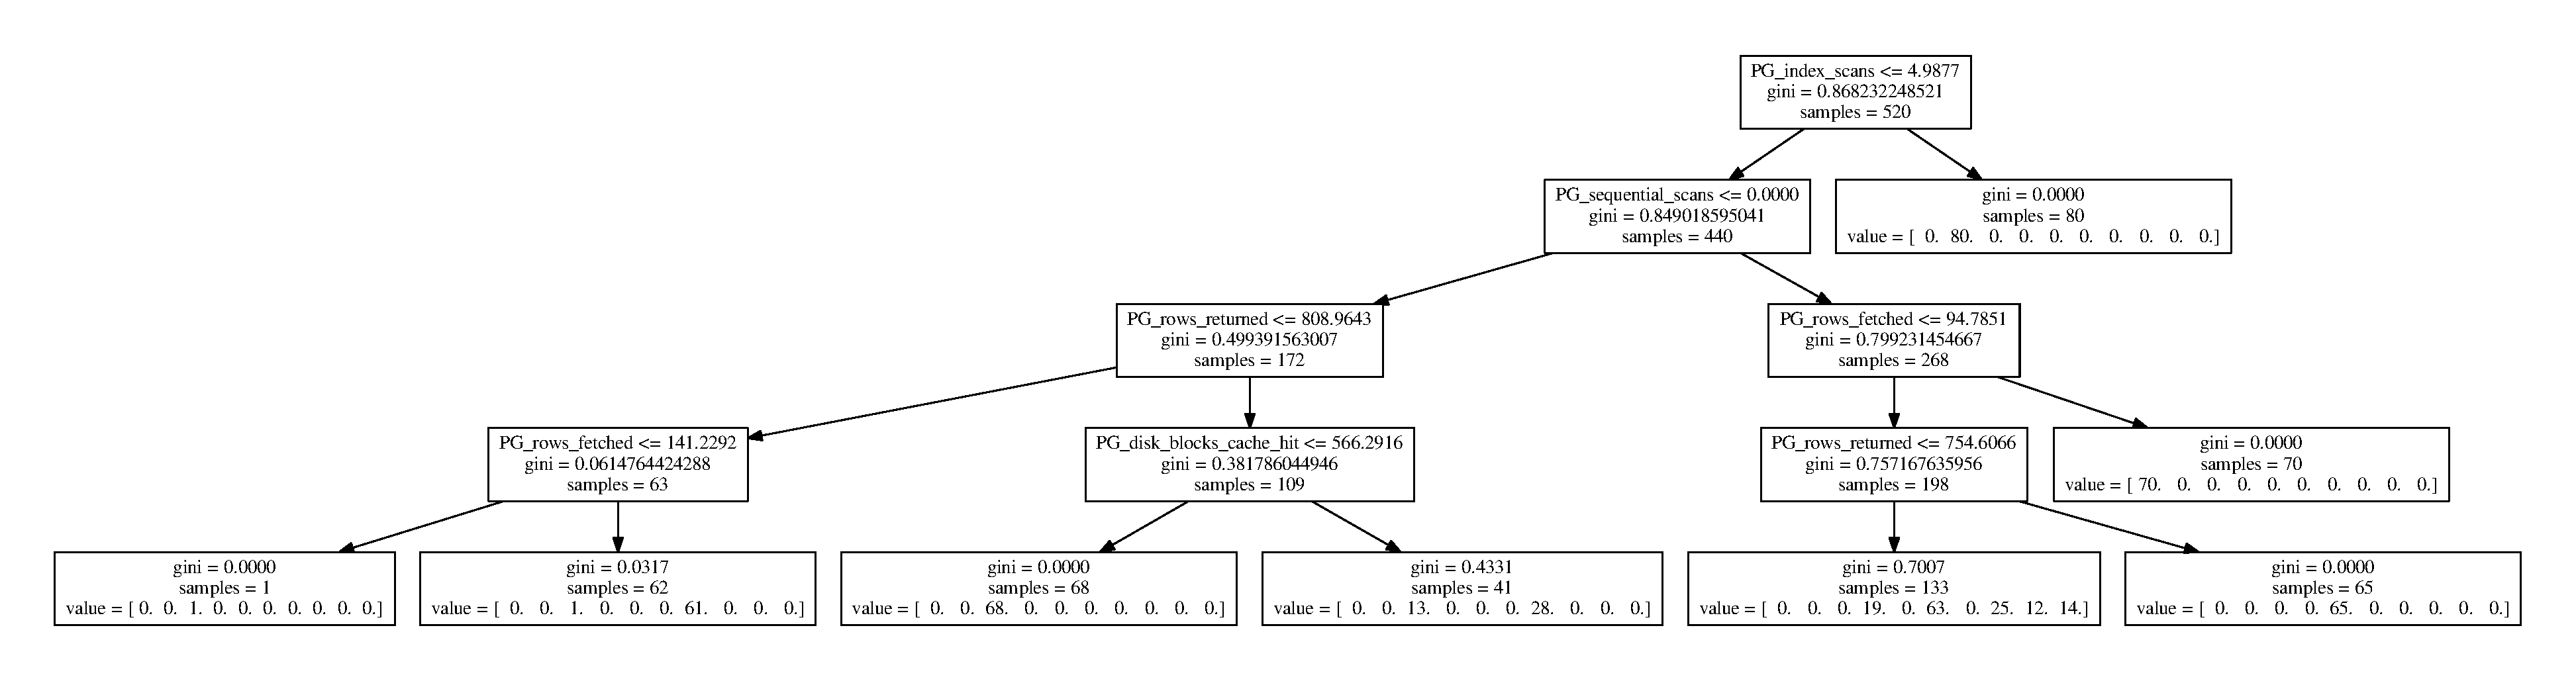
\includegraphics[width=\linewidth]{figure/tree_4.pdf}}
    \caption{Decision tree with max depth set to 4.}
    \label{fig:tree_4}
\end{figure*}

\begin{figure*}[h!]
    \centering
    \fbox{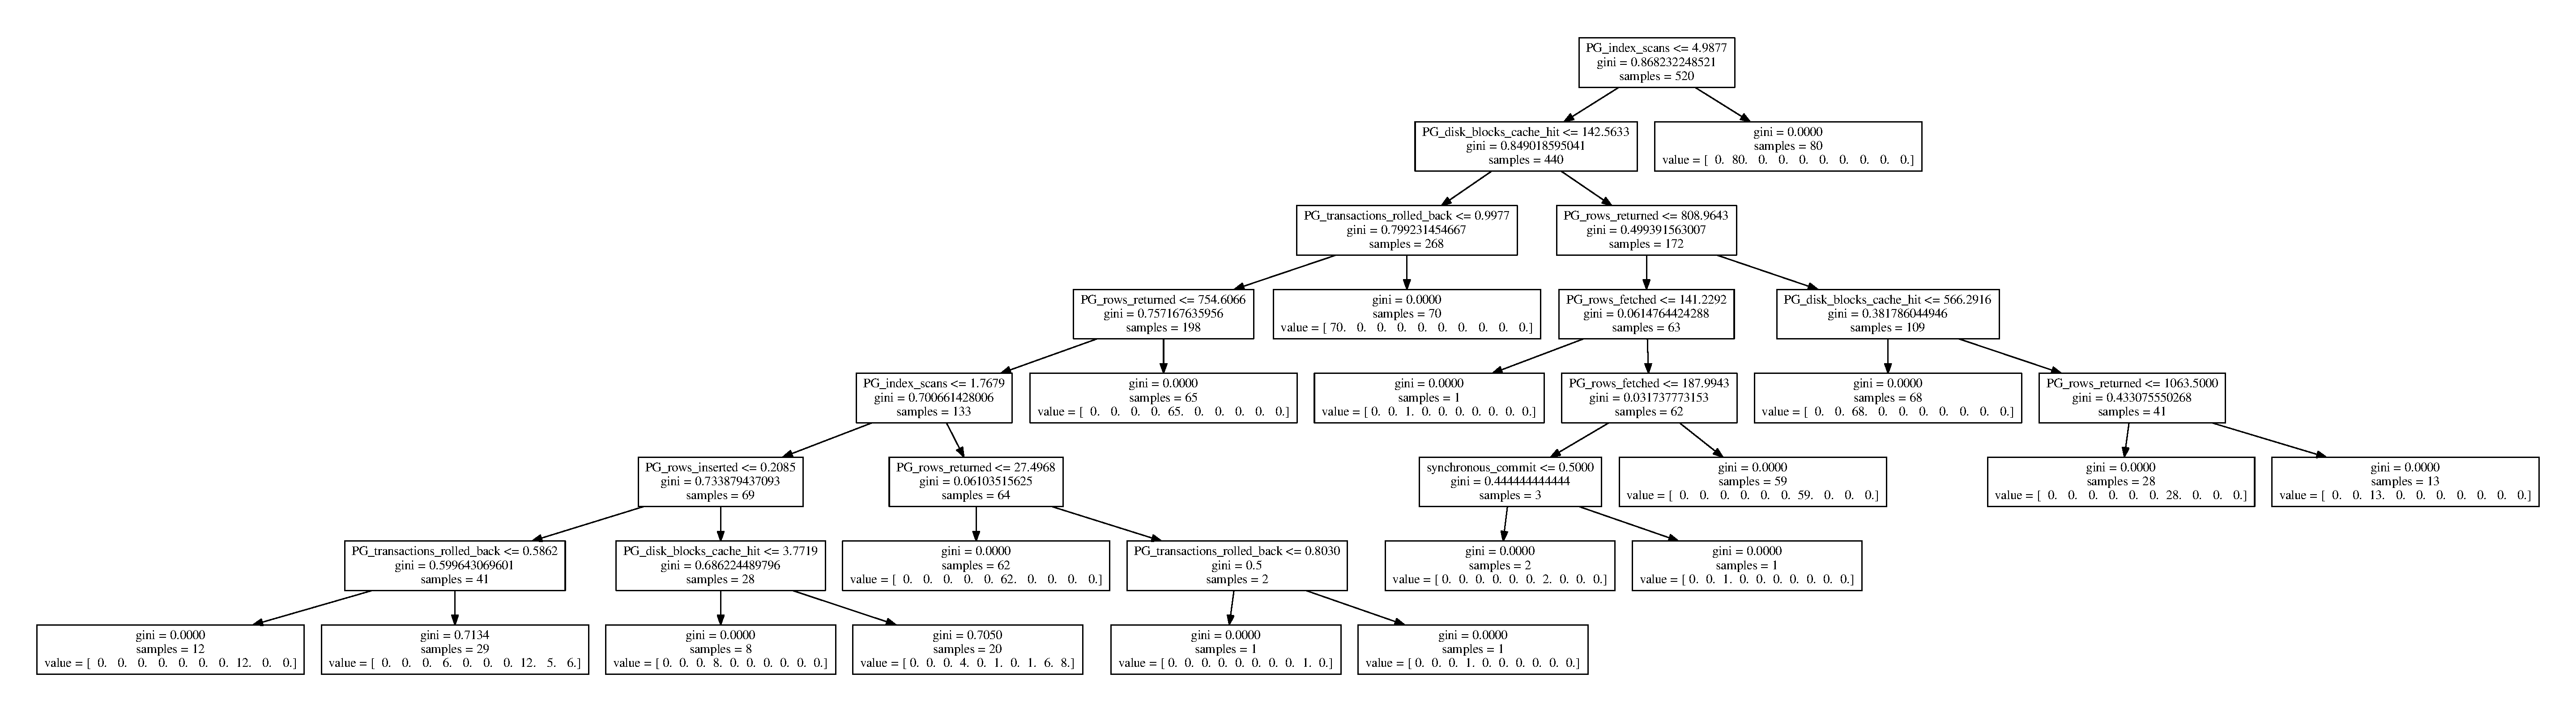
\includegraphics[width=\linewidth]{figure/tree_7.pdf}}
    \caption{Decision tree with max depth set to 7.}
    \label{fig:tree_7}
\end{figure*}

The clusters found by each algorithm can be seen in
\cref{fig:clusters}. We also calculated common clustering metrics such
as homogeneity, completeness, and V-measure. These results can be
found in \cref{fig:clustering-metrics}. From the results, we notice
immediately that DBSCAN does not work well with our data. Indeed, it
does not find any distinct clusters at all. However, K-Means and Ward
Agglomerative Clustering algorithms perform well. 
Both of these algorithms require number of clusters as a 
parameter. 
However, this is not a restriction for our problem as we
know the number of benchmarks - and hence the number of clusters -
that we have.

In addition to evaluating clustering algorithms, we also evaluated
Support Vector Machines, a supervised classifier. While real-world
data will not be labeled and hence a supervised classifier cannot be
used, it is still useful to see how effective our features are in
discriminating between benchmarks. Using a simple two-fold
cross-validation, we found that a simple SVM with an RBF kernel
achieved 86\% precision but with a very high standard deviation of
28\%. However, this is still a very strong result as it indicates that
our features effectively separate our data into our desired
classes. 
We plan to validate the classifier on more sophisticated heterogeneous 
real-world workloads as part of our stretch goal.

The immediate next step is to build an estimator that allows us to address the
second goal of this project. We already have the infrastructure required
for collecting metrics and features required for solving this problem.
We plan to explore different machine learning algorithms to solve this
problem in the coming weeks.

\begin{figure*}[h!]
    \centering
	\subfloat[\label{fig:dt_depth}]{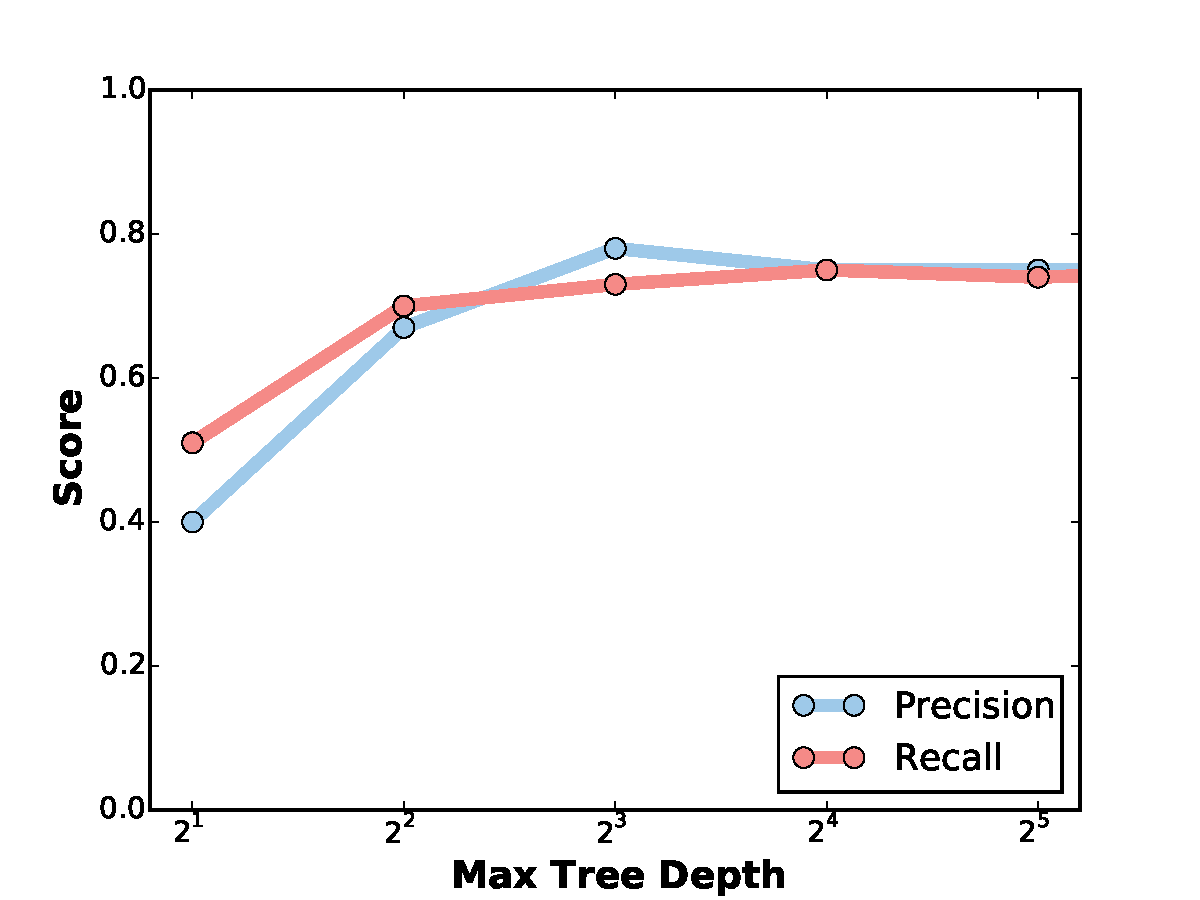
\includegraphics[width=0.4\linewidth]{figure/depth.pdf}}
	\subfloat[\label{fig:dt_leaves}]{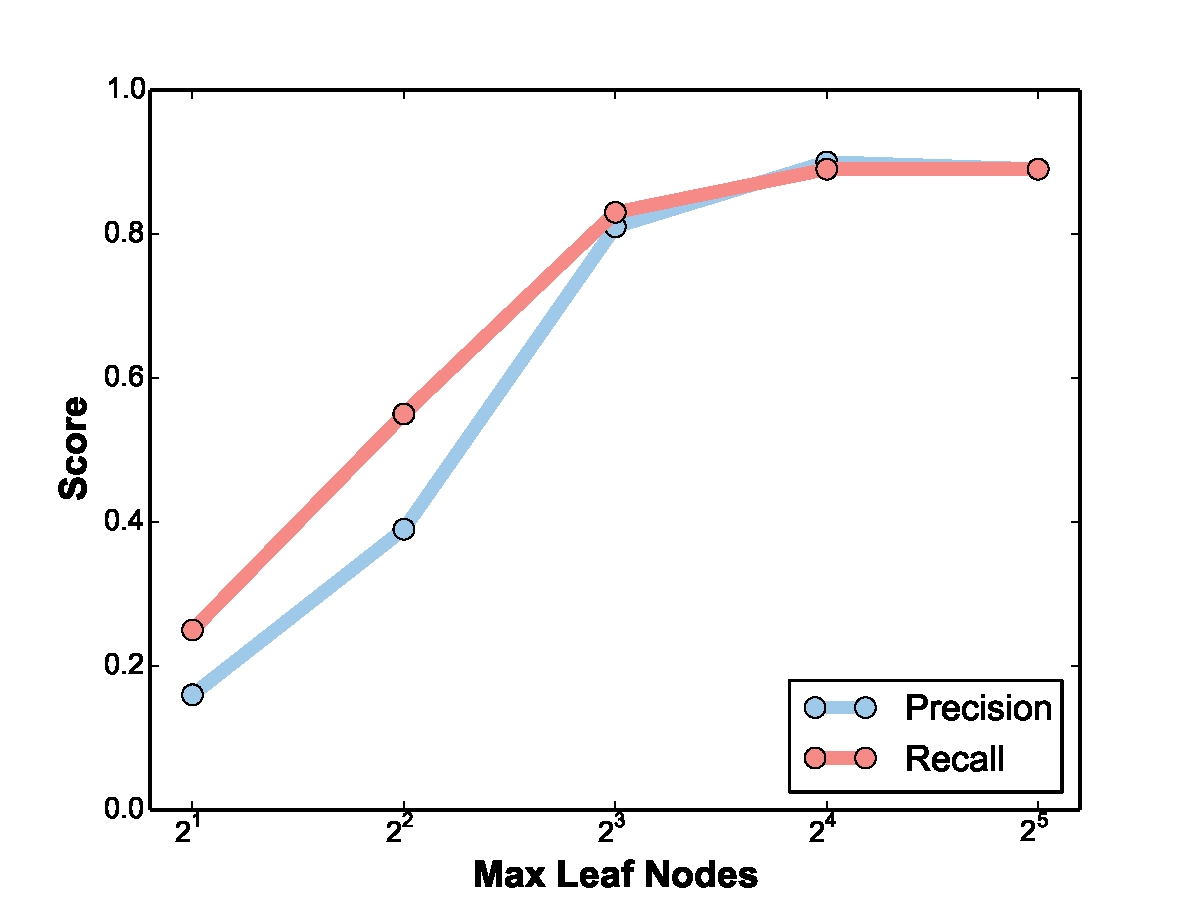
\includegraphics[width=0.4\linewidth]{figure/leaves.pdf}}
	\caption{Impact of max depth and max leaf nodes on the accuracy of the
    decision tree.}
\end{figure*}

\begin{table}[h!]
\centering
\small{
  \centering
  \begin{tabular}{l|llll} 
	\toprule
   		Class &  Precision  &  Recall &  F1-score  &  Support  \\    
    \midrule
		0.0   &    1.00   &   0.00   &   1.00   &     84   \\
        1.0   &    0.99   &   1.00   &   0.99   &     74   \\
        2.0   &    0.98   &   0.99   &   0.98   &     81   \\
        3.0   &    0.54   &   0.39   &   0.45   &     18   \\
        4.0   &    1.00   &   1.00   &   1.00   &     69   \\
        5.0   &    1.00   &   0.99   &   0.99   &     70   \\
        6.0   &    1.00   &   0.95   &   0.97   &     60   \\
        7.0   &    0.41   &   0.95   &   0.57   &     19   \\
        8.0   &    0.00   &   0.00   &   0.00   &     17   \\
        9.0   &    0.56   &   0.52   &   0.54   &     27   \\
    \midrule
Avg / Total   &    0.90   &   0.91   &   0.90   &    519   \\
   \bottomrule
   \end{tabular}
 }
%\nocaptionrule
\caption{Per-class accuracy of the default decision tree.}
\label{tab:dt_stats}
\end{table}


% -----------------------------------------------
% Estimated number of clusters: 10
% Homogeneity: 0.614
% Completeness: 0.628
% V-measure: 0.621
% Adjusted Rand Index: 0.429
% Adjusted Mutual Information: 0.606
% [2 8 9 ..., 3 1 1]
% Silhouette Coefficient: 0.111
% 
% Metrics for Affinity Propogation
% -----------------------------------------------
% Estimated number of clusters: 88
% Homogeneity: 0.654
% Completeness: 0.317
% V-measure: 0.427
% Adjusted Rand Index: 0.067
% Adjusted Mutual Information: 0.248
% [72  8 22 ..., 30 74 39]
% Silhouette Coefficient: 0.082
% 
% Metrics for Mean-Shift
% -----------------------------------------------
% Estimated number of clusters: 2
% Homogeneity: 0.012
% Completeness: 0.368
% V-measure: 0.024
% Adjusted Rand Index: -0.001
% Adjusted Mutual Information: 0.010
% [0 0 0 ..., 0 0 0]
% Silhouette Coefficient: 0.517
% 
% Metrics for Ward Agglomerative Clustering
% -----------------------------------------------
% Estimated number of clusters: 10
% Homogeneity: 0.589
% Completeness: 0.635
% V-measure: 0.611
% Adjusted Rand Index: 0.458
% Adjusted Mutual Information: 0.581
% [0 4 5 ..., 4 2 6]
% Silhouette Coefficient: 0.097
